% !TeX root = Chapter_08_Slides.tex
% Chapter 8 lecture slides — Risk Finance and Alternative Risk Transfer
% Instructor-resource series; model deck: Chapter_01_Slides.tex
\documentclass[11pt, aspectratio=169]{beamer}
\usepackage{tikz}
\makeatletter
\def\input@path{{./}{../slides/}}
\makeatother
\usepackage{erm_beamer_theme}
\usepackage{amsmath,amssymb}
\graphicspath{{../rscripts/chapter8/}}

\title[ERM Ch.\,8]{Risk Finance and Alternative Risk Transfer}
\subtitle{Enterprise Risk Management, Second Edition --- Chapter 8}
\author{Martin F.\ Grace}
\institute{University of Iowa\\[2pt] Tippie College of Business\\[2pt] Vaughan Institute of Risk Management}
\date{June 2026}

\begin{document}

\begin{frame}[plain]
\titlepage
\end{frame}

\begin{frame}{Learning Objectives}
\begin{itemize}
  \item Map the \alert{risk financing spectrum} from full retention through traditional insurance to alternative risk transfer.
  \item Calculate \alert{total cost of risk (TCOR)} for retention versus transfer, including expense loads, capital costs, and administration.
  \item Design retention programs (deductibles, SIRs) that cut TCOR while respecting risk appetite.
  \item Evaluate captive insurance companies: structure, domicile, and tax treatment.
  \item Assess ART products: finite risk, multi-trigger policies, risk retention groups.
  \item Analyze catastrophe bonds and ILS --- trigger design, basis risk, and when capital markets beat reinsurance.
\end{itemize}
\end{frame}

\section{Opening Case: The Bond That Paid When the Earth Moved}

\begin{frame}{March 11, 2011 --- Tokyo Disneyland}
\begin{itemize}
  \item 2:46 p.m.: a magnitude 9.0 earthquake --- the largest ever recorded in Japan --- strikes off the T\=ohoku coast.
  \item Oriental Land Company (OLC) operates Tokyo Disneyland and DisneySea on \emph{reclaimed land} in Tokyo Bay: $\sim$25--30 million guests per year, everything concentrated on one shoreline strip.
  \item The structures held. The \alert{ground} didn't: liquefaction buckled pavements, ruptured utilities, sank and tilted whole sections. Both parks went dark.
  \item The liquefaction risk was no surprise --- it sat in OLC's catastrophe models and engineering reviews for years.
\end{itemize}
\end{frame}

\begin{frame}{The Decision Made in 2006}
\begin{itemize}
  \item Five years earlier, OLC's treasury had sold a \textyen 10 billion \alert{catastrophe bond} through an SPV called Midori Ltd.
  \item Investors bought the notes; proceeds sat in a collateral trust. No qualifying quake $\Rightarrow$ investors get principal back plus premium coupons.
  \item The trigger was \alert{parametric}: payment depended entirely on seismograph readings at specified monitoring stations --- no claims adjuster, no loss inspection, no negotiation.
  \item OLC had looked at seismic maps, reinsurance pricing, and a capital market willing to bear Japanese earthquake risk --- and pre-arranged financing for a catastrophe it hoped would never come.
\end{itemize}
\end{frame}

\begin{frame}{The Payout --- and the Lesson}
\begin{itemize}
  \item The recorded ground motion crossed the contractual thresholds. The numbers were unambiguous: \alert{the bond triggered}.
  \item $\sim$\textyen 10 billion arrived within weeks --- settled like a bond, because it was one. Investors lost principal; OLC funded reconstruction.
  \item Tokyo Disneyland reopened in late March --- faster than outside observers expected.
  \item A slightly different earthquake could have produced heavy damage \emph{without} a triggering reading. Basis risk didn't disappear; it just didn't bind that day.
\end{itemize}
\medskip
\begin{block}{The decision problem}
In 2006, reinsurance was available and familiar. Why would a theme park operator go to the \emph{capital markets} instead --- and accept a trigger that pays on physics, not on damage?
\end{block}
\end{frame}

\section{Risk Financing Follows Risk Control}

\begin{frame}{Control Changes the Distribution; Financing Pays for What Remains}
\begin{itemize}
  \item \alert{Risk control} (Ch.\,7) modifies loss frequency and severity --- the distribution itself shifts.
  \item \alert{Risk financing} leaves the distribution alone; it decides \emph{who bears the consequences, and when}.
  \item OLC's bond did not make the ground firmer. It made sure that when the ground failed, money arrived.
  \item Decisions occur at three levels:
  \begin{itemize}
    \item \textbf{Strategic} --- what share of enterprise risk to retain versus transfer
    \item \textbf{Portfolio} --- how to allocate the financing budget across risk categories
    \item \textbf{Individual} --- retain, transfer, or hybrid (deductibles, caps) per exposure
  \end{itemize}
\end{itemize}
\end{frame}

\begin{frame}{Why Financing Creates Value: Five Channels}
In an MM world, paying an insurer's expense load destroys value. Each channel exploits a specific friction:
\begin{itemize}
  \item \textbf{Cost minimization} --- retain predictable losses; avoid paying 25--40\% loads on losses you could finance yourself.
  \item \textbf{Cash flow timing} --- retention delays outflows until losses occur; insurance accelerates them for budget certainty.
  \item \textbf{Tax efficiency} --- premiums deduct immediately; self-insured losses only when paid. Captives add planning room (within anti-abuse limits).
  \item \textbf{Reduced distress costs} --- tail transfer is contingent capital arriving when internal resources are under maximum strain. The OLC channel.
  \item \textbf{Managerial focus} --- executives improvising catastrophe financing are not running the business.
\end{itemize}
\end{frame}

\section{The Risk Financing Spectrum}

\begin{frame}{The Spectrum: Cost versus Retained Volatility}
\begin{columns}[T]
\column{0.62\textwidth}
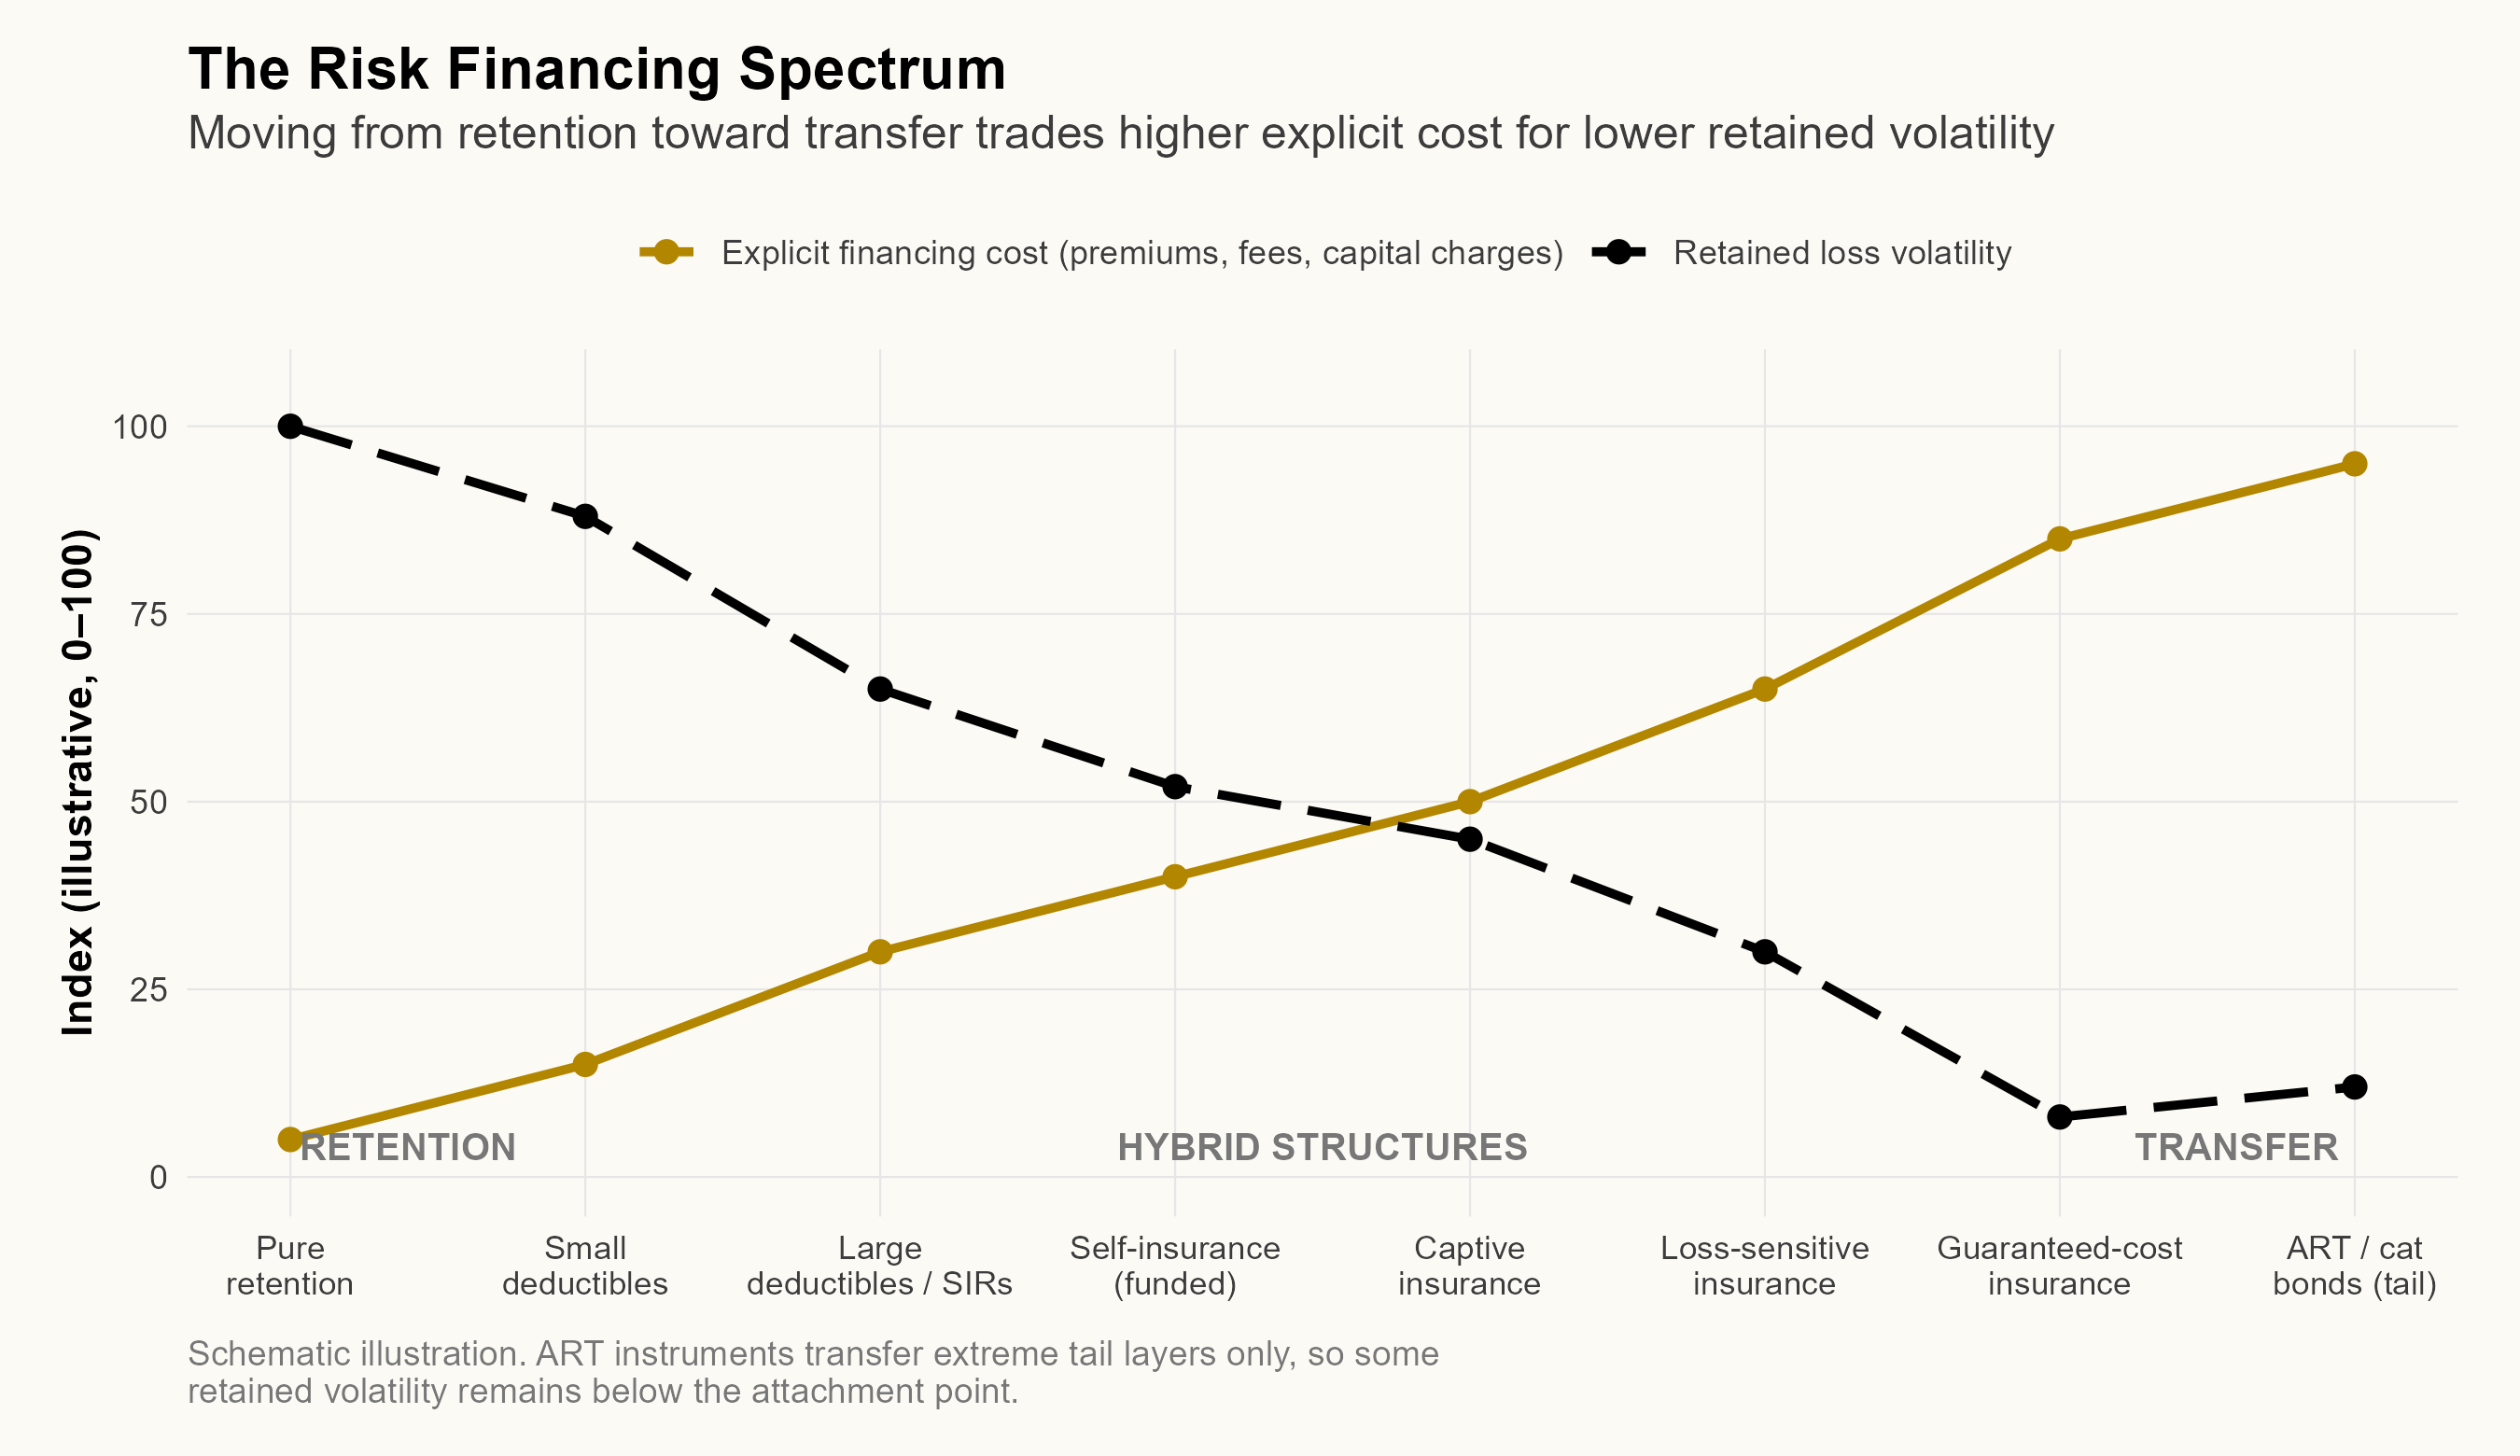
\includegraphics[width=\textwidth]{c8_financing_spectrum.png}
\column{0.34\textwidth}
\begin{itemize}
  \item Each step from retention toward transfer raises \alert{explicit cost} and lowers \alert{retained volatility}
  \item Volatility reduction is a service --- insurers and investors charge for it
  \item ART wrinkle: instruments at the high-cost end transfer only extreme tail layers, so volatility remains below the attachment point
\end{itemize}
\end{columns}
\end{frame}

\begin{frame}{Stops Along the Spectrum}
\begin{columns}[T]
\column{0.48\textwidth}
\begin{itemize}
  \item \textbf{Pure retention} --- no premiums, maximal volatility, full claims control
  \item \textbf{Small deductibles} --- 5--15\% premium savings; kills nuisance claims
  \item \textbf{Large deductibles \& SIRs} --- \$250K--\$1M+ retentions cut premiums 30--50\%
  \item \textbf{Funded self-insurance} --- actuarial reserves, TPA claims, stop-loss
\end{itemize}
\column{0.48\textwidth}
\begin{itemize}
  \item \textbf{Captive} --- a licensed insurance subsidiary formalizing retention
  \item \textbf{Loss-sensitive insurance} --- retro rating ties final premium to experience
  \item \textbf{Guaranteed cost} --- maximum budget certainty, highest load
  \item \textbf{ART} --- cat bonds, sidecars, ILWs, finite structures at the far end
\end{itemize}
\end{columns}
\medskip
SIR vs.\ deductible: under an SIR the insured pays claimants \emph{directly} before coverage attaches; a deductible is advanced by the insurer and reimbursed.
\end{frame}

\begin{frame}{The Expense Load}
\[
\text{Premium} = \text{Expected Loss} \times (1 + \text{Expense Load})
\]
\begin{itemize}
  \item Load components: acquisition 10--15\%, administration 10--15\%, profit and contingencies 5--10\% --- typically a \alert{25--40\% markup} over expected losses.
\end{itemize}
\medskip
\begin{exampleblock}{Example: why large deductibles save money}
\begin{itemize}
  \item Ground-up cover on \$1M expected losses at a 40\% load: premium \$1.4M.
  \item Retain the first \$500K per occurrence: expected retained \$600K; excess premium \$600K (\$400K of transferred losses at a 50\% load --- excess layers carry higher loads).
  \item Total cost falls \$1.4M $\rightarrow$ \$1.2M: \alert{\$200K saved} by not paying a load on losses the firm can finance itself --- in exchange for retained-layer volatility.
\end{itemize}
\end{exampleblock}
\end{frame}

\section{Retention versus Transfer: The Core Decision}

\begin{frame}{The Fundamental Cost Comparison}
\begin{itemize}
  \item Retention cost $=$ expected retained losses $+$ capital charge $+$ administration.
  \item Transfer cost $=$ premiums $+$ residual retained losses $+$ brokerage and fees.
\end{itemize}
\begin{exampleblock}{Worked example: \$2M expected losses, VaR(95\%) \$3.5M, $k = 10\%$}
\begin{itemize}
  \item \textbf{Retain:} \$2.0M losses $+$ \$350K capital cost ($\$3.5\text{M} \times 0.10$) $+$ \$200K admin $= \$2.55$M
  \item \textbf{Transfer:} \$2.7M premium ($1.35\times$) $+$ \$135K broker $+$ \$100K retained $= \$2.935$M
  \item Retention saves \alert{\$385K (13\%)} --- but exposes the firm to \$3.5M+ outcomes.
  \item If appetite caps annual loss volatility at \$3M, retention is \alert{infeasible} regardless of expected savings. The appetite constraint, not the cost comparison, binds.
\end{itemize}
\end{exampleblock}
\end{frame}

\begin{frame}{The Optimal Retention Level}
\[
\min_{R} \; \text{TCOR}(R) = E[L(R)] + k \cdot C(R) + P(R) + \text{Admin}(R)
\quad \text{s.t.} \quad \text{VaR}_{0.95}(R) \le \text{Appetite}
\]
\medskip
\begin{center}\small
\begin{tabular}{@{}lrrrrr@{}}
\toprule
\textbf{Retention} & \textbf{Retained loss} & \textbf{Cap.\ cost} & \textbf{Premium} & \textbf{Total} & \textbf{VaR(95\%)} \\
\midrule
\$0 (full ins.) & 0 & 0 & 2{,}025 & 2{,}025 & $\approx 0$ \\
\$500K & 400 & 72 & 1{,}485 & 1{,}957 & 2{,}800 \\
\$1M & 700 & 126 & 1{,}080 & 1{,}906 & 3{,}500 \\
\bottomrule
\end{tabular}
\end{center}
\medskip
\begin{itemize}
  \item (\$000s; load 35\%, capital at 150\% of retained losses, $k = 12\%$, appetite VaR $\le$ \$4M.)
  \item Each dollar of expected loss moved to retention saves its 35-cent load but costs 18 cents of capital charge --- retention wins until \alert{appetite stops it}. Optimum: \$1M.
\end{itemize}
\end{frame}

\begin{frame}{Five Decision Rules}
\begin{itemize}
  \item \textbf{Retain high-frequency, low-severity} --- the law of large numbers makes outcomes nearly certain; the load buys nothing. Fleet damage, employee health claims.
  \item \textbf{Transfer low-frequency, high-severity} --- catastrophic exposures warrant transfer despite expensive pricing. Pharma product liability; \alert{earthquake for a Tokyo Bay theme park}.
  \item \textbf{Cap retention by capacity} --- aggregate annual retention $\le$ 5--10\% of net worth or 15--20\% of pre-tax earnings.
  \item \textbf{Transfer non-core, retain core} --- insurers hold advantages in D\&O; the firm controls product quality and safety better than any insurer.
  \item \textbf{Evaluate correlation in aggregate} --- uncorrelated retentions are safer than line-by-line analysis suggests; correlated ones are more dangerous.
\end{itemize}
\end{frame}

\section{Traditional Risk Financing: Commercial Insurance}

\begin{frame}{What the Expense Load Buys}
\begin{block}{Three economic functions of insurance}
\textbf{Risk pooling} --- thousands of independent exposures make the insurer's aggregate predictable. \quad
\textbf{Claims expertise} --- cost containment, litigation management, repair networks; savings can exceed the insurer's entire fee. \quad
\textbf{Contingent capital} --- pre-arranged financing activated by loss; the same function OLC bought from bond investors.
\end{block}
\medskip
\begin{itemize}
  \item \textbf{Property}: all-risks forms, exclusions for flood/quake; business interruption rides on the form.
  \item \textbf{CGL}: \alert{occurrence} basis --- coverage attaches when injury occurred; long-tail exposure.
  \item \textbf{Workers' comp}: statutory benefits, exclusive remedy; predictable $\Rightarrow$ the standard line for large deductibles and self-insurance.
  \item \textbf{Professional liability}: \alert{claims-made} basis --- tail coverage needed when switching insurers.
\end{itemize}
\end{frame}

\begin{frame}{Loss-Sensitive Structures and the Market Cycle}
\begin{columns}[T]
\column{0.48\textwidth}
\textbf{Blending retention and transfer}
\begin{itemize}
  \item \textbf{Experience rating} --- premiums adjust to the insured's own history (the EMR)
  \item \textbf{Retrospective rating}:
\end{itemize}
\[
\text{Retro} = (\text{Basic} + \text{Conv.\ Losses}) \times \text{Tax Mult.}
\]
\begin{itemize}
  \item bounded by minimum ($\sim$60--70\%) and maximum ($\sim$125--140\%) premiums
  \item \textbf{Dividend plans} --- 20--40\% of premium returnable for excellent experience
\end{itemize}
\column{0.48\textwidth}
\textbf{Hard and soft markets}
\begin{itemize}
  \item \textbf{Soft}: abundant capacity, aggressive pricing, broad terms
  \item \textbf{Hard}: capital impairment $\Rightarrow$ rates up 10--50\%+, terms narrowed, capacity withdrawn
  \item Hardenings: 9/11, Katrina, 2017--2021
  \item Strategic lesson: hold a stable program designed around your own capacity --- don't chase the cycle
\end{itemize}
\end{columns}
\end{frame}

\section{Self-Insurance}

\begin{frame}{Self-Insurance Is Structured Retention --- Not ``Going Bare''}
A true program has actuarial funding, professional claims administration, integrated loss control, aggregate protection, and regulatory compliance.
\medskip
\begin{itemize}
  \item Five conditions favor it --- successful programs usually satisfy all:
  \begin{itemize}
    \item \textbf{Scale}: 500+ employees (WC) or 250+ vehicles --- the law of large numbers operates internally
    \item \textbf{Financial capacity}: required reserves $\le$ 15--20\% of net worth
    \item \textbf{Superior risk management}: outperform the average that commercial rates price to --- and keep the difference
    \item \textbf{Load savings exceed admin}: drop the 25--40\% load, add 5--15\% administration; the net must be positive
    \item \textbf{Cash flow value}: investment opportunities exceed the risk-free rate
  \end{itemize}
\end{itemize}
\end{frame}

\begin{frame}{Program Structure}
\begin{itemize}
  \item \textbf{Funding}: pre-funded reserves or pay-as-you-go; letters of credit (1--3\%) or surety bonds (2--5\%) satisfy state security requirements without tying up cash.
  \item \textbf{Claims}: internal staff (only for very large programs), \alert{TPAs} (\$150--\$400 per claim or 8--12\% of incurred losses), or \alert{fronting} (a licensed insurer issues the policy; the insured keeps the economic risk).
\end{itemize}
\begin{exampleblock}{Aggregate stop-loss: capping the bad year}
\begin{itemize}
  \item Expected WC losses \$3M; aggregate coverage attaches at 130\% $=$ \$3.9M.
  \item Actual losses hit \$5M $\Rightarrow$ stop-loss insurer pays the \$1.1M above the attachment.
  \item Premium for the layer: typically 5--15\% of the covered layer.
\end{itemize}
\end{exampleblock}
\end{frame}

\section{Captive Insurance Companies}

\begin{frame}{The Captive Concept}
\begin{block}{Definition}
A \alert{captive} is a licensed insurer owned and controlled by its insureds, formed primarily to cover the parent's risks --- retention formalized inside an insurance company structure. Roughly 7,000 operate worldwide.
\end{block}
\medskip
\begin{itemize}
  \item Eliminates the commercial insurer's profit and overhead; pays only incremental administration, regulation, and reinsurance.
  \item Premium accumulates as captive surplus --- the \alert{``float'' stays home}.
  \item Writes coverage commercial markets price punitively or refuse: terrorism, recall, cyber.
  \item Buys reinsurance directly at wholesale, skipping an intermediary layer.
  \item Possible tax advantages --- premium deductibility, favorable insurer taxation (next slide's caveats).
\end{itemize}
\end{frame}

\begin{frame}{Captive Structures and Domiciles}
\begin{columns}[T]
\column{0.48\textwidth}
\textbf{Structures}
\begin{itemize}
  \item \textbf{Single-parent}: one owner, max control; capital \$250--500K+, operating \$75--250K+/yr
  \item \textbf{Group}: unrelated firms pool homogeneous risks --- hospitals pooling malpractice
  \item \textbf{Protected cell (PCC)}: legally segregated cells share infrastructure, not solvency; \$25--75K/yr --- the mid-market entry point
  \item Rent-a-captive; agency captives (conflict-prone)
\end{itemize}
\column{0.48\textwidth}
\textbf{Domiciles}
\begin{itemize}
  \item \textbf{Vermont}: 800+ captives, sophisticated regulator, 0.4\% premium tax capped at \$200K
  \item \textbf{Bermuda}: 700+, no corporate income tax, direct reinsurance access --- but CFC complications
  \item Delaware, Cayman, EU domiciles (passporting)
  \item Choice turns on tax, regulatory quality, cost, reinsurance access
\end{itemize}
\end{columns}
\end{frame}

\begin{frame}{Captive Tax: Where the Economics Can Break}
\begin{itemize}
  \item Deductibility requires the arrangement to be \emph{insurance} under \emph{Helvering v.\ Le Gierse} (1941): genuine \alert{risk transfer} \emph{and} \alert{risk distribution} (enough pooling for the law of large numbers).
  \item Single-parent captives struggle with distribution; fixes include 30\%+ unrelated third-party business, pools, or many operating subsidiaries.
  \item \textbf{The \S\,831(b) election}: ``micro-captives'' (premiums $\le$ \$2.85M, 2025) pay tax on investment income only --- legitimate for genuine small captives, heavily abused as estate-planning shelters. IRS re-designated abusive structures as listed transactions in 2024.
  \item Offshore captives are typically CFCs; Subpart F can pull insurance income into current U.S.\ taxation --- one reason U.S.\ domiciles have grown at the offshore centers' expense.
  \item The touchstones never change: \alert{real risk transfer, arm's-length pricing, adequate capital, business purpose beyond tax}.
\end{itemize}
\end{frame}

\section{Alternative Risk Transfer}

\begin{frame}{Finite Risk: Transferring Timing, Not Underwriting}
\begin{itemize}
  \item Insurer's maximum loss capped at 110--125\% of premium; multi-year terms (3--10 yrs); premiums set above expected losses, the excess accruing interest in an \alert{experience account}.
\end{itemize}
\begin{exampleblock}{Calloway Industries: 5-year finite product liability cover}
\begin{itemize}
  \item Premium \$2M/yr (\$10M total); expected losses \$6M; insurer cap \$12M (120\%); 4\% interest credit.
  \item At expiry: positive balance refunded; deficit up to \$2M repaid by Calloway; beyond the cap is the reinsurer's loss.
\end{itemize}
\end{exampleblock}
\begin{itemize}
  \item Uses: loss smoothing for earnings guidance, structured funding of long-tail reserves, capital relief.
  \item \alert{Caution}: contracts must transfer genuine risk (ASC 944) or they are deposits --- finite deals were central to the AIG/Gen Re accounting scandals.
\end{itemize}
\end{frame}

\begin{frame}{Multi-Trigger Programs and Risk Retention Groups}
\begin{columns}[T]
\column{0.48\textwidth}
\textbf{Multi-trigger \& integrated}
\begin{itemize}
  \item Pays only when two events coincide: utility quake cover requiring M7.0+ \emph{and} a 25\% stock drop --- prices at 40--60\% of conventional cover
  \item Logic: external capital is needed only when damage coincides with impaired financing --- the distress channel, contract-engineered
  \item Integrated programs bundle 5 lines under one aggregate retention: 15--25\% cheaper because perils are imperfectly correlated
\end{itemize}
\column{0.48\textwidth}
\textbf{Risk retention groups}
\begin{itemize}
  \item Liability Risk Retention Act (1986): member-owned liability insurers operate nationwide under \alert{one state license}
  \item Born of the mid-1980s liability crisis; $\sim$240 RRGs today --- malpractice, product liability, commercial auto
  \item Liability lines only; member ownership and industry homogeneity required
  \item Failure mode: underpricing and under-reserving in the early years
\end{itemize}
\end{columns}
\end{frame}

\section{Catastrophe Bonds and ILS}

\begin{frame}{Cat Bond Mechanics}
\begin{block}{The structure --- every element solves a contracting problem}
Sponsor pays premium to an \alert{SPV}; the SPV issues notes and deposits proceeds in a \alert{collateral trust} (Treasury money funds). Investors earn the money-market rate \emph{plus} a risk spread of 300--1{,}000 bp. No trigger $\Rightarrow$ principal returns at maturity. Trigger $\Rightarrow$ collateral flows to the sponsor.
\end{block}
\medskip
\begin{itemize}
  \item The sponsor's economic cost is the \alert{spread}, not the full coupon --- the collateral earns the money-market rate on its own.
  \item Versus reinsurance: \alert{fully collateralized} (no counterparty risk after a market-wide cat) and \alert{multi-year} (3--5 yrs, locking pricing across the cycle).
  \item ILS market $>$ \$100B; cat bonds $\sim$\$45B outstanding.
\end{itemize}
\end{frame}

\begin{frame}{Pricing the Investor's Side}
\begin{exampleblock}{Example: \$300M Florida hurricane bond, SOFR + 650 bp}
\begin{itemize}
  \item SOFR at 4\% $\Rightarrow$ running yield 10.5\%. Modeled annual trigger probability: 2\%.
  \item Expected one-year return (coupon paid even in a trigger year):
\end{itemize}
\[
E[R] = 0.98 \times 10.5\% + 0.02 \times (-100\% + 10.5\%) \approx 8.3\%
\]
\begin{itemize}
  \item The 2\% expected principal loss consumes about a fifth of the coupon --- what remains is compensation for tail risk that arrives \emph{suddenly and totally}.
\end{itemize}
\end{exampleblock}
\begin{itemize}
  \item Investor appeal: returns driven by hurricanes and earthquakes, not rates and earnings --- near-zero correlation with stocks and bonds.
\end{itemize}
\end{frame}

\begin{frame}{Trigger Design: Basis Risk versus Moral Hazard}
\begin{center}\small
\begin{tabular}{@{}llll@{}}
\toprule
\textbf{Trigger} & \textbf{Basis risk} & \textbf{Moral hazard} & \textbf{Settlement} \\
\midrule
Indemnity & None & Highest & Slow (loss development) \\
Industry loss & Two-way & Low & Moderate (PCS estimate) \\
Parametric & Largest & None & \alert{Fast} (physics, no adjustment) \\
Modeled loss & Moderate & Low & Moderate \\
\bottomrule
\end{tabular}
\end{center}
\medskip
\begin{itemize}
  \item \alert{Basis risk}: the gap between what the sponsor loses and what the bond pays. \alert{Moral hazard}: the sponsor's ability to influence payout.
  \item Midori was parametric: payment on seismograph readings, settled in weeks. The 2011 quake crossed the thresholds \emph{and} caused severe damage --- but a near-miss quake could have left OLC with losses and no recovery.
  \item Handle basis risk the Coastal REIT way: measure it, price it, and place indemnity layers where index and portfolio diverge most --- don't pretend it's absent.
\end{itemize}
\end{frame}

\begin{frame}{When ILS Beats Reinsurance --- and When It Doesn't}
\begin{columns}[T]
\column{0.48\textwidth}
\textbf{Advantages}
\begin{itemize}
  \item Multi-year committed capacity --- insulated from renewal repricing
  \item Capital markets replenish faster than reinsurer balance sheets after a cat
  \item Collateralization kills counterparty risk
  \item Speed: OLC financed reconstruction while a conventional claim would still be in documentation
\end{itemize}
\column{0.48\textwidth}
\textbf{Limitations}
\begin{itemize}
  \item Basis risk on non-indemnity triggers
  \item Transaction costs \$0.5--2M per issue --- bonds below \$100M are rare
  \item 3--6 month lead time
  \item Concentrated in well-modeled perils; cyber and terrorism mostly out of reach
\end{itemize}
\end{columns}
\medskip
A precision tool, not a general substitute for insurance.
\end{frame}

\section{Total Cost of Risk Optimization}

\begin{frame}{TCOR: The Common Currency}
\[
\begin{aligned}
\text{TCOR} ={}& \text{Retained Losses} + \text{Transfer Costs} + \text{Admin Costs} \\
&+ \text{Indirect Costs} + \text{Cost of Risk Capital}
\end{aligned}
\]
\begin{center}\small
\begin{tabular}{@{}lrrrr@{}}
\toprule
\textbf{Strategy} & \textbf{Retained} & \textbf{Premium} & \textbf{TCOR} & \textbf{VaR(95\%)} \\
\midrule
Guaranteed cost & 0 & 2{,}700 & \textbf{2{,}750} & $\approx 0$ \\
\$250K deductible & 600 & 1{,}890 & \textbf{2{,}715} & 1{,}200 \\
\$500K deductible & 900 & 1{,}485 & \textbf{2{,}723} & 1{,}800 \\
\$1M SIR & 1{,}350 & 878 & \textbf{2{,}684} & 2{,}600 \\
Self-ins.\ + stop-loss & 2{,}000 & 400 & \textbf{3{,}070} & 3{,}200 \\
\bottomrule
\end{tabular}
\end{center}
\medskip
\begin{itemize}
  \item (Brennan Industrial, \$000s.) Unconstrained optimum: the \$1M SIR. With appetite capped at VaR \$2M, the \$250K deductible wins --- and the constraint \alert{costs \$31K/yr}, a price worth showing the board explicitly.
  \item Full self-insurance is \emph{dominated}: more retention is not always better.
\end{itemize}
\end{frame}

\begin{frame}{The Portfolio View Pays}
\begin{itemize}
  \item Line-by-line optimization ignores diversification: if property and liability correlate at 0.3 rather than 1.0, combined retained volatility is far below the sum of the parts.
  \item Example: independent analyses recommend \$2.25M of total retention across WC, property, and liability. Joint optimization with the correlation structure supports $\sim$\$3M --- about a third more --- saving \alert{an additional \$180K/yr} in expense loads.
  \item The same logic cuts both ways: lines that move \emph{together} (the Maersk cascade, Ch.\,6) should be retained more cautiously than line-by-line analysis implies.
  \item In practice (the chapter's three cases): GlobalTech's high-retention program saves 8.2\% of TCOR; MidState's malpractice RRG saves 40\% versus a hard market; Coastal REIT's layered reinsurance-plus-cat-bond tower saves 16\% --- and locks three years of pricing.
\end{itemize}
\end{frame}

\begin{frame}{Discussion Questions}
\begin{enumerate}
  \item Walk through the mechanics of a catastrophe bond --- sponsor, SPV, collateral trust, trigger, spread. Why is the sponsor's economic cost the spread rather than the full coupon? Use the OLC/Midori transaction to illustrate.
  \item Compare the four trigger types on basis risk, moral hazard, and settlement speed. Why did a parametric trigger suit OLC --- and what risk did OLC accept in choosing it?
  \item Describe the conditions under which retention beats transfer. Which is most often the binding one in practice, and why?
  \item A coastal insurer can buy \$200M of hurricane protection as traditional reinsurance (\$22M/yr, indemnity, annual renewal) or a 3-year cat bond (\$26M/yr, industry trigger, $\sim$20\% basis risk). Which would you choose --- and under what circumstances is the \emph{more expensive} cat bond preferable?
\end{enumerate}
\end{frame}

\end{document}
